\documentclass[10pt,conference,compsocconf]{IEEEtran}

\usepackage{hyperref}
\usepackage{amsmath}
\usepackage{amsfonts}
\usepackage{float}
\usepackage{graphicx}	% For figure environment



\begin{document}
% \title{Toward breast cancer personalized medicine \\ A machine learning perspective}
\title{Global gene expression analysis: determine hormone signalling activation in human breast cancer samples}

\author{
  Gautier Pialla, Ambroise Renaud, Emrick Sinitambirivoutin\\
  gautier.pialla@epfl.ch, ambroise.renaud@epfl.ch, emrick.sinitambirivoutin@epfl.ch\\
  \textit{Department of Computer Science, EPFL, Switzerland}
}

\maketitle
% Topic
% Purpose
% Scope
% Results
% Conclusion
\begin{abstract}

70\% of breast cancers can be classified as estrogen receptor positive (ER+). Recent evidences describe tumor as a very complex and heterogeneous disease, highlighting the importance of taking into consideration inter- and intra-tumor variability. Patient-derived xenografts (PDXs) emerged as promising and clinically-relevant preclinical model able to recapitulate the clinical settings.
One promising way to estimate human cells receptivity to hormones is to analyse patient genes expression.
In this document, we present a set of machine learning algorithms and features selection techniques to classify human cells implanted into mice according to their hormone receptivity by using only their gene expression.
According to the results of our study, we show that this method can be used to classify patient's cells receptivity to hormones.



\end{abstract}



\section{Introduction}
A challenging problem which arises in the medicine field is giving the right drug to the right person.
Currently almost all the patients who are diagnosed with ER+ breast cancer undertake endocrine therapies. 

Many studies have shown that understanding the receptivity of breast cancer tumor cells to hormones could help finding more specific treatments for a given patient and at the end improve their cure rates. One of the main challenge of this approach is to be able to determine the receptivity of a given tumor to hormones. 
Little is known about how normal epithelial breast cells are affected by hormonal stimulation. In order to decipher the genetic signature imposed by different hormones, PDX models coming from different patients were treated with different hormones, the injected mammary glands retrieved and the transcriptomic profile of these samples analyzed by RNAseq. This approach allows us to study in a clinicaly-relevant context what are the main genes whose expression is altered upon a hormonal stimulation. 

Given a dataset composed of mice groups, hormones that they have been exposed to and their resulting cells gene expression, the goal of this work is to apply a machine learning tool in order to set up a classifier that would discriminate and recognize what are the actual hormone responses in patients, using the data that was generated in our in vivo model (PDXs).

The final goal of this work is to propose a method to generalize the classification models trained on this dataset to a human unlabelled dataset.

\section{Feature selection and visualization}

\subsection{The dataset}

The dataset has been collected at the \emph{EPFL Brisken Laboratory, Switzerland} and is part of a PhD research project. It contains information related to 15004 genes describing a total of 29 samples collected from mice which were exposed to 3 different hormonal treatments.

The dataset contains the following information:
\begin{itemize}
    \item Unique identifier for each mouse sample (containing the information about which hormones they have been exposed to).
    \item Samples gene expressions for 15004 different genes with their names.
\end{itemize}

The dataset have been preprocessed in order to extract the labels from the samples identifiers and then normalized. At the end each row contains the identifier of the mouse, its genes and its label.

Two approaches of normalization were done, first we normalized the features with respect to the rows (scaling each mouse given the mean value of the features and its standard deviation). The other approach was normalizing the features with respect to the columns (scaling each feature given the mean value of this feature over the dataset and its standard deviation).

\subsection{Feature selection}

With only $N=29$ samples and more than 15000 features ($D = 15004$), one of the main challenge in order to train models that achieves good performance is to reduce the number of features that we consider for the classification. To reduce the dimensions of our dataset, we tried two main approaches. The first one was to use Principal Component Analysis (PCA) in order to map our data from the D-dimensional space to a K-dimensional space, $K \ll D$, that has maximum variance and then we computed the most meaningful features that contributed to each components. The other approach was to train a Logistic Regression with $_1$ regularisation. As the $l_1$ norm introduces sparsity we then looked at the features that were selected (non-zero weighed) after the training. We found almost the same features for both kind of normalization.

Here are the results that we got with each methods:
\begin{itemize}
    \item 
    \textbf{PCA}: We projected our feature space into a 2-D space (Component 1 with $62\%$ of the variance and Component 2 with $13\%$ of the variance). We then selected the 50 more representative features of each of those two components. We end up with 100 features to represent our data.
    \item 
    \textbf{Logistic regression with $_1$ norm}: We trained a Logistic classifier with different number of iteration and then choose the one maximizing sparsity while maintaining a good accuracy on our test set. With this method we were able to remove $97.9\%$ of our features and only select 785 relevant features for our model (with the regularisation term $\lambda=0$ and $\texttt{num\_iter}=10000$).
\end{itemize}

In the main time to fine tune our feature selection, we also took into consideration a list of features (genes) that were considered by a domain expert as relevant. By combining these information with the features that we extracted with the two previous methods we found the following correspondence:

\begin{table}[H]
    \centering
    \begin{tabular}{|p{3cm}|p{1.5cm}|p{2.6cm}|}
        \hline
          \textbf{Type of feature selection} & \textbf{Number of features} & \textbf{Percentage of common features with domain expert} \\
         \hline
           Domain expert & 56 & 100\%\\
           \hline
           PCA & 1000 & 0.04\%\\
           \hline
           $l_1$ Logistic regression & 785 & 89\%\\
         \hline
    \end{tabular}
    \caption{Feature selection methods comparison with domain expert selection}
    \label{tab:feature_selection_table}
\end{table}

As we can see in Table \ref{tab:feature_selection_table}, the selected features from regularized Logistic regression seems to be much more relevant as they perfectly match with the one selected by a domain expert. In our following experiments we will only consider the 56 expert selected features.

\subsection{Feature visualization}

One other important aspect in order to understand our data is to be able to visualize it. Doing so is a good way to see if we observe clusters.

\subsubsection{Principal components analysis}

As a two component PCA can preserve most of the information of our original D dimension dataset (here 75\% of the variance) , we used it to visualise our sample in 2 dimensions.

\begin{figure}[H]
    \centering
    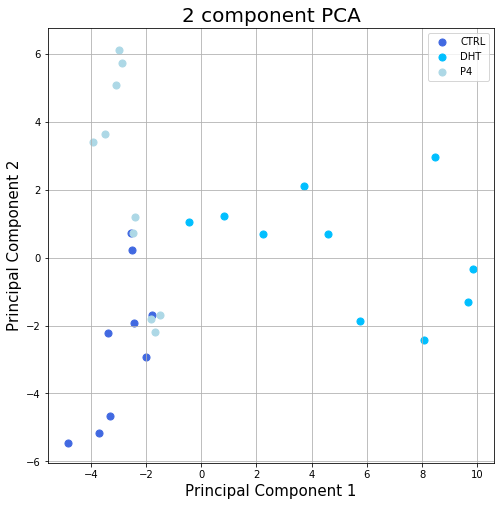
\includegraphics[width=0.48\columnwidth]{figures/PCA_feature_normalized.png}
    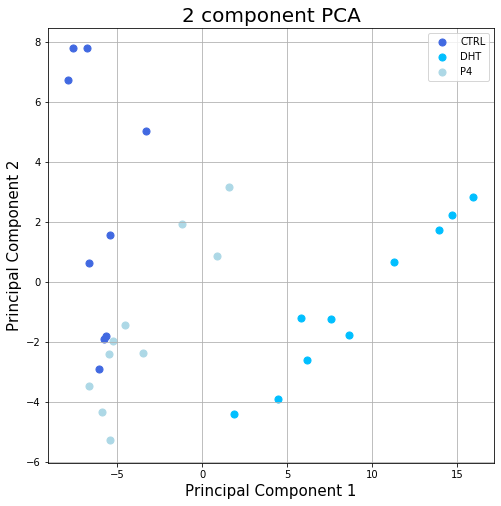
\includegraphics[width=0.48\columnwidth]{figures/PCA_sample_normalized.png}
    \caption{PCA with two different normalization methods. (left) with respect to features, (right) with respect to samples.}
    \label{fig:pca}
\end{figure}

Both plots show distinct clusters, but some points are really closed to each others. This information will need to be taken into account while reading the result of our models.

\subsubsection{Gaussian Mixture Model (GMM)}

An other way to visualise how our clusters can be constructed is to use Gaussian Mixture Models \cite{Murphy:2012:MLP:2380985}. In our case, we see that it would be nice to have elliptical clusters that data points can belong to more than one cluster (e.g : returning a probability array instead of a cluster index). Both of the problems can be addressed by using mixture model. We can see on Figure \ref{fig:gmm} the result that we obtained using GMM on the PCA that we obtained earlier.

\begin{figure}[H]
    \centering
    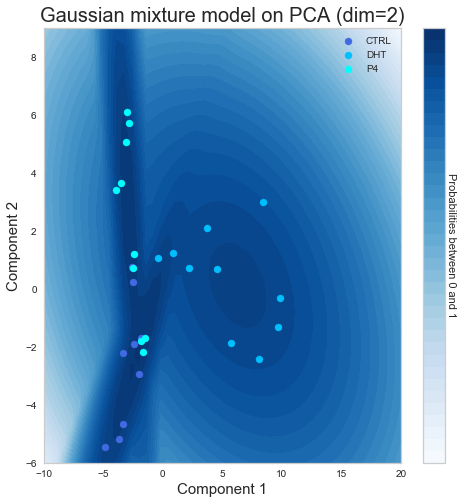
\includegraphics[width=0.48\columnwidth]{figures/Gaussian_mixture_3_feature_normalized.png}
    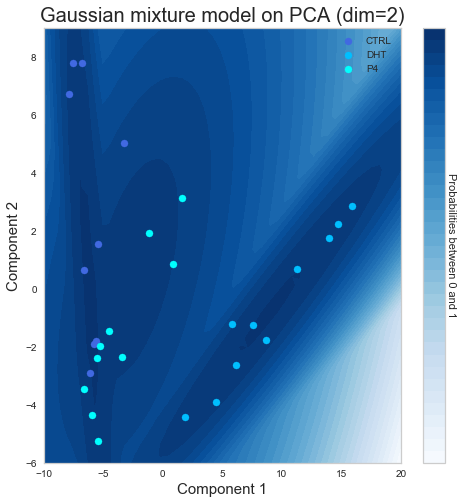
\includegraphics[width=0.48\columnwidth]{figures/Gaussian_mixture_3_sample_normalized.png}
    \caption{Gaussian Mixture Model visualization. (left) with respect to features, (right) with respect to samples}
    \label{fig:gmm}
\end{figure}


\section{Models and Methods}
\subsection{Algorithms and Models}

\subsubsection{Logistic regression}

Logistic regression is one of the most fundamental and widely used Machine Learning Algorithms. It is not a regression algorithm but a probabilistic classification model.

In a binary classification problem, given a training set $\mathbf{X_{train}}$ and the corresponding labels $\{0, 1\}$, the logistic regression algorithm learns the weight vector $\mathbf{w}$ and a scalar $\mathbf{w_0}$ to predict the probability of the two class labels given a test example $\mathbf{x} = \mathbf{x}_{test}$ \cite{epfl_ml_cs}:

\begin{align*}
p(0 | \mathbf{x}) &= \sigma(\mathbf{x^\top}  \mathbf{w} + w_0)
\\
p(1 | \mathbf{x}) &= 1 - \sigma(\mathbf{x^\top}  \mathbf{w} + w_0)
\end{align*}

In  the case of multi-class classification this term can be generalized to the following formula:
\begin{equation*}
\mathbb{P}(b_{i} = j | \mathbf{x}_{i}, \mathbf{W}) = \frac{e^{\mathbf{x}_{i}^{T}\mathbf{w}_{j}}}{\sum_{k=1}^{C}e^{\mathbf{x}_{i}^{T}\mathbf{w}_{k}}}
    \label{eqn:plr}
\end{equation*}

This problem can be solved by minimizing the negative log likelihood estimator:

$ f: \mathbb{R}^{d*C} \rightarrow \mathbb{R}, f(W) = -\log p(y | X, W)$ : 
\begin{align*}
    \mathbf{\hat{W}}_{ML} \in \text{arg}\min_{\mathbf{W}}\{f(\mathbf{W}) \}
\end{align*}

\subsubsection{K-Nearest Neighbors}

Another algorithm that can be applied to our classification problem is K-Nearest Neighbors (K-NN). It's a \emph{lazy learning} algorithm, which means that it does not have a \emph{training} phase like the previous algorithm. Generalization of the training data is delayed until a query is made to the system. In the previous algorithms, the model tries to learn a discriminating function from the training examples, so it generalize the training data before receiving queries, while KNN directly "memorize" the model to interact with it.

In our implementation the K-NN algorithm use the \emph{Minkowski distance} defined as:
\begin{align*}
    D\left(X,Y\right)=\left(\sum_{i=1}^n |x_i-y_i|^p\right)^{1/p} \text{with p=2}
\end{align*}

Given an input vector $\mathbf{x}$ from the dataset, K-NN algorithm assign it to the class in which the majority of its k nearest neighbors belong\cite{ml_python}.


Figure \ref{fig:knn} shows decision boundaries of the 3 different labels on the mice dataset in the space of the 2 principal components. To computed these probabilities, model was trained on the whole dataset and it predicted using the graph mesh coordinates as testing points.

\begin{figure}[H]
    \centering
    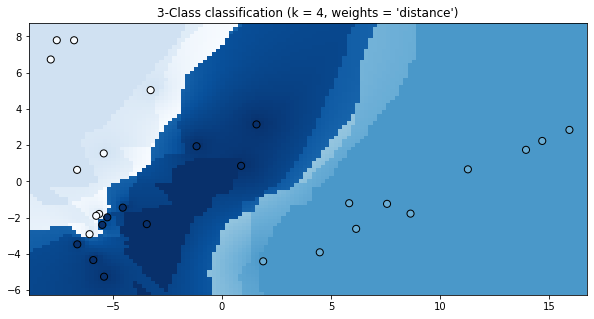
\includegraphics[width=\columnwidth]{figures/knn-4.png}
    \caption{Probabilistic decision boundaries of K-NN on the mice dataset}
    \label{fig:knn}
\end{figure}

\subsubsection{Decision Tree}

From the \emph{root node} to a \emph{leaf}, a binary \emph{"Yes"/"No"} choice is applied to a single feature. The travel from the root node to the leaf is achieved sequentially. The idea behind this is that the feature space is partitioned by hyperplane parallel to the axes. The partitioning is done by answering several questions such as \emph{"is feature $x_j < \theta$"} where $\theta$ is a threshold (the \emph{split criterion}). At each node $t$ the matrix $\mathbf{X}$ is split in two sets : $\mathbf{X_{t, N}}$ and $\mathbf{X_{t, Y}}$ where $N$ stands for "No" and $Y$ stands for "Yes" which is the answer to the question related to the feature at the current node. \cite{ml_python}

The aim of this algorithm is to select which feature to test. This is done by defining an \emph{impurity} criterion, here \emph{gini} is used to chose the right feature/class at each node, $\mathbf{X_{t, N}}$ and $\mathbf{X_{t, Y}}$ have to be class-homogeneous compared to $\mathbf{X}$.

\begin{figure}[H]
    \centering
    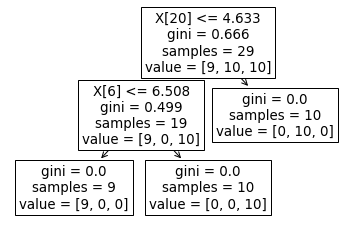
\includegraphics[width=0.6\columnwidth]{figures/dt_plot.png}
    \caption{Decision Tree trained on the mice dataset}
    \label{fig:decision_tree}
\end{figure}

Figure \ref{fig:decision_tree} shows that the most important genes to determine the hormone receptivity are GPR88 (X[20]) and KLK3 (X[6]). It can be noticed that the algorithm stopped drawing the tree after classifying training points with a good enough accuracy with respect to the features selected.

\subsubsection{Random Forest}
A \emph{Random forest} is like an ensemble of decision trees. The aim of this algorithm is to generalize the decision tree model in order to avoid overfitting. The algorithm is defined as follows :
\begin{enumerate}
    \item Create $b$ training sets using \emph{bootstrap} (chose $n$ samples from $\mathbf{X}$ with remplacement).
    \item Train a decision tree on each training set.
    \item Each prediction is saved.
    \item The final prediction is assigned to the class label by majority vote.
\end{enumerate}

\subsection{Validation and Hyper-parameter tuning}

The following Tables show the parameters selected using 5-fold cross-validation and a grid-search.

\textbf{Logistic regression}

\begin{table}[H]
    \centering
    \begin{tabular}{|c|c|c|}
        \hline
        \textbf{Algorithm} &  \textbf{Penalty} &  $\lambda$ \textbf{(regularization rate)}\\\hline
        Logistic regression&$l_{2}$    & 1.0  \\\hline
                Logistic regression&$l_{1}$    & 1.0  \\\hline
    \end{tabular}
    \caption{Hyper-parameters for regression algorithms}
    \label{tab:param_regression}
\end{table}
\vspace{-1.2cm}

\textbf{K-NN}

\begin{table}[H]
    \centering
    \begin{tabular}{|c|c|c|}
        \hline
        \textbf{Algorithm} &\textbf{k} & \textbf{\# PCA components}\\\hline
        KNN& 2 & 9   \\\hline
    \end{tabular}
    \caption{Hyper-parameters for lazy learning algorithms}
    \label{tab:param_lazy}
\end{table}
\vspace{-0.5cm}

\textbf{Random forest}

For the random forest algorithm in Table \ref{tab:param_tree}, the number of bootstrap has been set by an empirical evidence.

\begin{table}[H]
    \centering
    \begin{tabular}{|c|c|}
        \hline
        \textbf{Algorithm} &\textbf{\# Bootstrap}\\\hline
        Random forest& 100 \\\hline
    \end{tabular}
    \caption{Hyper-parameters for tree algorithms}
    \label{tab:param_tree}
\end{table}
\vspace{-0.5cm}


\textbf{Gaussian mixture model}

In Table \ref{tab:param_cluster}, elbow method or silhouette coefficient could have been used, but since we know the number of classes we set the number of clusters to 3. This value could not have been chosen using cross-validation based on accuracy because Gaussian mixture model is a unsupervised clustering method. The number of components for the PCA is 2 in order to visualize the clusters in a 2-dimensional space.

\begin{table}[H]
    \centering
    \begin{tabular}{|c|c|c|}
        \hline
        \textbf{Algorithm} &\textbf{\# Clusters} & \textbf{\# PCA components}\\\hline
        Gaussian mixture model& 3 & 2   \\\hline
    \end{tabular}
    \caption{Hyper-parameters for clustering algorithms}
    \label{tab:param_cluster}
\end{table}
\vspace{-1.2cm}


\section{Results}

\subsection{Testing}

All the algorithm were able to predict labels on the mice dataset with an accuracy score of at least 0.80\% for the best models, using K-fold cross-validation (k=5), the average accuracy score and the F1-score for each algorithm is presented in Table \ref{tab:result_acc}. However, logistic regression without feature selection offers poor results due to the dimensions of the features space.

\begin{table}[H]
    \centering
    \begin{tabular}{|c|c|c|}
    \hline
    \textbf{Algorithm}      &\textbf{Accuracy}&\textbf{F1-Score} \\\hline
    Logistic regression ($l_{2}$)    &      0.926 & 0.919      \\\hline
    Logistic regression ($l_{2}$) (no feature selection)   &      0.653 & 0.586      \\\hline
    K-NN                        &      0.933    &  0.928     \\\hline
    K-NN (no feature selection) &      0.28     &  0.20     \\\hline
    Decision tree               &      0.880    &  0.871   \\\hline
    Decision tree  (no feature selection)&      0.75 &    0.72   \\\hline
    Random forest               &     0.933   &  0.928    \\\hline
    Random forest  (no feature selection)&     0.647  &  0.616    \\\hline
    
    \end{tabular}
    \caption{Algorithms Accuracies and F1-Scores}
    \label{tab:result_acc}
\end{table}
\vspace{-1cm}

\subsection{Prediction}

One of the goal of this project is to predict hormones receptivity with respect to the gene measurements on a human dataset. Because labeling these data is not as easy as labeling the mice dataset, we do not have the ground truth values of the labels. However we can try predicting labels and giving a confidence score as a probability value.

Figure \ref{fig:pred_results} show a representation of our results predicted with our best logistic regression model in a 2 dimensional space using PCA. Size of labels represent the confidence score of the prediction (predicted probabilities).

\begin{figure}[H]
    \centering
    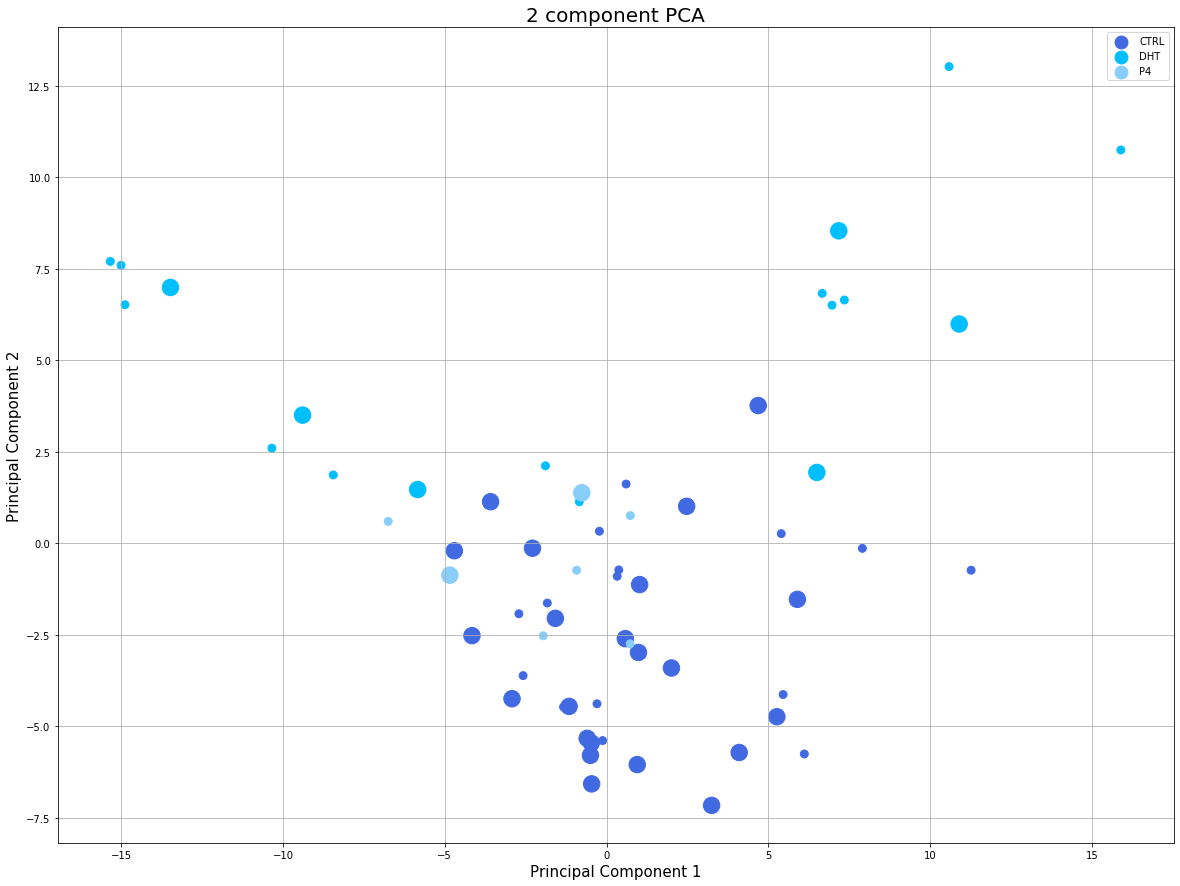
\includegraphics[width=0.8\columnwidth]{figures/predicted_pca.png}
    \caption{PCA of logistic regression predictions}
    \label{fig:pred_results}
\end{figure}

All these predictions are summarized in a CSV file in order to be validated by an expert. Once validated, further discussions can be made to validate if a model trained on a mice dataset can be generalized to a human dataset.

\section{Discussion}
From the short review above, key findings emerge: on the mice dataset it is possible to predict hormone receptivity with a relatively good confidence.

Furthermore, we have shown that feature processing and feature selection are important part of the machine learning pipeline. It helped increasing our models accuracies and also permitted to visualize the training points on a 2-dimensional space. The approach utilised suffer from the lack of training samples to be able to use more advanced techniques such as deep learning or even optimize our hyper-parameters in a less biased way.

Moreover it cannot be stated if the models can be generalized to humans since these data are not yet labelled. 

\section{Conclusions}
By using feature reduction, multi-class classification algorithms, testing/validation techniques and hyper-parameters tuning methods, we were able to apply some of the machine learning tools that we studied in the course to achieve good accuracy on this project.

Machine learning techniques can be a good starting point for a better understanding of key factors of breast cancer and to pave the way for a more informed choice when it comes to decide a treatment to be administered to ER+ breast cancer. Future research can take into account machine learning as an innovative tool to analyze hormone-driven transcriptomic profiles derived by PDX models. We can then try to apply this new methods in order to better classify and treat ER+ breast cancer patients.

\bibliographystyle{IEEEtran}
\bibliography{literature}

\end{document}
